\documentclass{article}
\usepackage[utf8]{inputenc}
\usepackage{url}
\usepackage{graphicx}
\graphicspath{ {./} }

\title{Assignment 21}
\author{Xiaoting Li (xil139) \\
Ziyu Zhang (ziz41) \\
Deniz Unal (des2014)}
\date{March 8 2019}

\begin{document}

\maketitle

\noindent
\textbf{32. Problem 8-6 from the CLRS text.}\\ \newline
\textbf{(a) For part a and b, it is essentially asking you to consider the adversarial strategy that answers so as to maximize the number of the original ways of merging two
sorted lists that are consistent with the answer. You will likely find Stirling��s approximation for n! useful.} \\ \newline
Answer: Given 2n numbers, we could first choose n numbers for list 1, and the n numbers remaining will be for list 2. So in all the number of ways to divide them into 2 sorted list is ${{2n}\choose{n}}$.  \\ \newline
Answer: The worst case of the number of comparisons is the height of the decision tree: number of comparisons = h.The decision tree will have more than  ${{2n}\choose{n}}$ leaves (since the permutations will be some of the leaves), and the tree will have no more than $2^h$ leaves, we get:${{2n}\choose{n}} \leq 2^h$, which is $h \geq lg{{2n}\choose{n}}$. Based on Stirling��s approximation, we have $lgn! = nlgn-n$, so $h\geq 2nlg2n -2n - 2(nlgn - n) = 2n-o(n)$ \\ \newline
\textbf{(b) For parts c and d, come up with a different adversarial strategy} \\ \newline
If two elements are consecutive in the sorted order and from opposite lists, then we don't have enough information about these two elements, and we have to get this through comparison to place them at the correct position using merge sort procedure.
Suppose we have 2 lists, where list A have a1,a2...an, and list B have b1,b2...bn, and the merged list is a1,b1,a2,b2...an,bn. And the final list will have 2n-1 pairs, where we need at least 2n-1 comparisons to get the final list. If the comparison is less than 2n-1, then we argue that at least one of the pairs has not been compared. And in the adversary, we pick a different order than the one we get from the comparison.\\ \newline
\textbf{(c) Explain why the bound that you get using the method proposed in parts a and b isn��t as good as the bound you get using an adversarial strategy. That is, in what way are you being too generous to the algorithm in parts a and b? In this generosity in the adversarial strategy or in its analysis?}\\ \newline The method we used in part a is not as good as the bound we get using an adversarial strategy, since it is not taking the comparisons that would be needed to merge. Adding these comparisons we have a tighter bound, so it is the generosity in the adversarial strategy.
\\ \newline
\textbf{33. We consider the distributed consensus problem as discussed in class and in the notes \url{http://homepage.divms.uiowa.edu/~ghosh/16612.week11.pdf}.}\\ \newline
\textbf{(a) Give a message passing algorithm that achieves distributed consensus if there are no processors failures.} \\ \newline
Answer: Since we need to achieve distributed consensus if there are no processors failures, we need to make sure that the algorithm meets the specification on termination, validity, and agreement. Let's say we have an iterative algorithm works as below. Each processor picks a favorite value (either 0 or 1), put this value in the message, and broadcast the message to all other processors. Since all messages will eventually be delivered, so when each processor receives the broadcast messages from other processors, it can change the favorite value based on the majority of the favorite values. Then repeat the same steps to do the broadcast again. We need to make sure the algorithm can get to termination. So we set a threshold $t$. As long as a processor achieves up to $t$ messages that have the same favorite value from at least $n/2$ processors ($n$ is the total number of processors), it means that the system achieves agreement. Then the process broadcast this value again and commits to the outcome. Using such algorithm, we make sure that every processors in the system will eventually decide and terminate, at the same time achieves agreement with valid values.  \\ \newline
\textbf{(b) Now assume that any 1 processor can experience a failure at any time (but $n-1$ of the processors will always work properly). You can think of a failure meaning that the machine is just turned off; The failed processors doesn��t do anything malicious. Show that there is no deterministic algorithm/protocol that can achieve distributed consensus in this setting.} \\ \newline 
Answer: From the hint, we learn that the way to prove this is similar to the way to prove the example in the note. Assume we look at one processor that sends messages to other processors and receives messages from other processors. \\ \newline
Case 1: Starting at bivalent state, the processor sends one message to processor $p$ to transit to state 1, and followed by a sequence of actions $e_1$ that lead to decision 1. The processor also sends one message to processor $q$ ($p\neq q$) to transit to state 0, and followed by a sequence of actions $e_0$ that lead to decision 0. If we let the processor sends message to $q$ and make $q$ crash, then the decision will be 1, which is a contradiction (state 0 can never transit to state 1).\\ \newline 
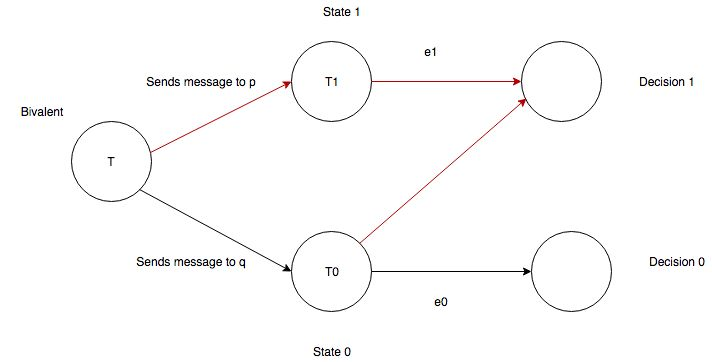
\includegraphics[width=0.9\columnwidth]{case1.jpg} \\\newline
Case 2: Starting at bivalent state, the processor sends one message to processor $p$ to transit to state 1, and followed by a sequence of actions $e_1$ that lend to decision 1. The processor also receives one message from processor $q$ ($p\neq q$) to transit to state 0, and followed by a sequence of actions $e_0$ that lead to decision 0. If we let the processor receive the message from $q$ and then make $q$ crash, then the decision will be 1, which is a contradiction(state 0 can never transit to state 1).\\ \newline
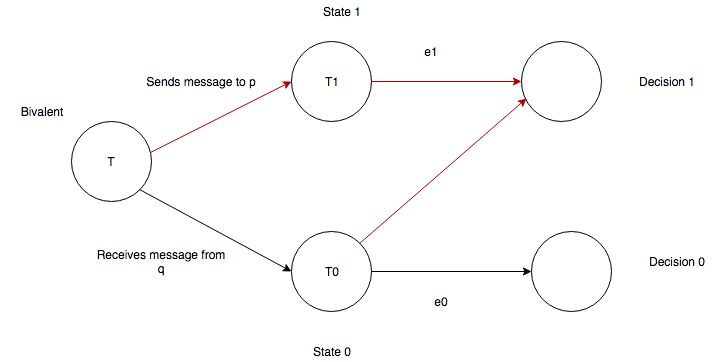
\includegraphics[width=0.9\columnwidth]{case2.jpg} \\ \newline
Case 3: Starting at bivalent state, the processor sends one message to processor $p$ to transit. The processor also receives one message from processor $p$. Then regardless of the order of these two operations, both of them will transit to the same intermediate state. However, we cannot decide whether the intermediate state should be 0 or 1.\\ \newline
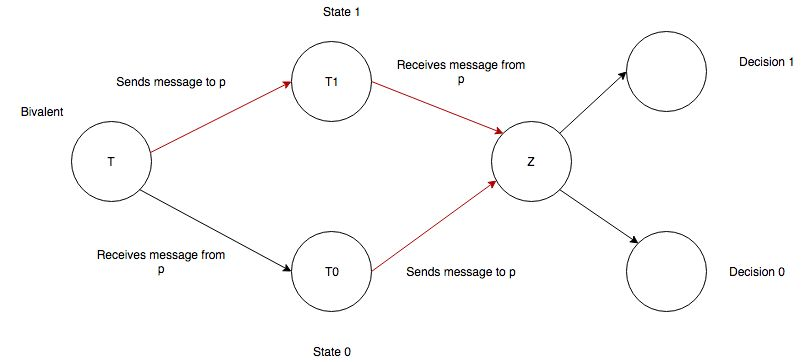
\includegraphics[width=0.9\columnwidth]{case3.jpg}\\ \newline 
\textbf{(c) Now assume that the transport layer connection additionally guarantees the in order delivery of messages between processors, like TCP. So if processor $i$ sends processor $j$ three messages, they will arrive at $j$ in the order that $i$ sent them. There is still no upper bound on the arrival time. Also there is no guarantee about the order of arrival of messages either sent to different processors, or sent from different processors. Now prove or disprove that there is a deterministic protocol that will achieve distributed consensus with up to one processor failure.}\\ \newline
Answer: We think there is no deterministic protocol that will achieve distributed consensus with up to one processor failure even the in order delivery of messages between processors are guaranteed. First, there is no guarantee about the order of arrival of messages either sent to different processors, or sent from different processors. Then we also know that there is no upper bound on the arrival time of the messages. So the system is still in an asynchronous environment. Those three cases in (b) can still happen. It is impossible to achieve consensus among deterministic processors even with one faulty processor. 

\end{document}
